\documentclass[11pt, oneside]{article}   	% use "amsart" instead of "article" for AMSLaTeX format
\usepackage{geometry}                		% See geometry.pdf to learn the layout options. There are lots.
\geometry{letterpaper}                   		% ... or a4paper or a5paper or ... 
%\geometry{landscape}                		% Activate for for rotated page geometry
%\usepackage[parfill]{parskip}    		% Activate to begin paragraphs with an empty line rather than an indent
\usepackage{graphicx}				% Use pdf, png, jpg, or eps§ with pdflatex; use eps in DVI mode
								% TeX will automatically convert eps -- pdf in pdflatex		
\usepackage{amssymb}
%\graphicspath{ {images/} }

\usepackage{mathtools}
\usepackage{enumitem}
\usepackage{setspace}
\usepackage{sidecap}

\usepackage{url}
\urlstyle{same}

\title{BME88A: EKG Preliminary Design Proposal}
\author{Eduardo Hirata, Henry Hinton, Pavle Jeremic}
%\date{}							% Activate to display a given date or no date

\begin{document}
\maketitle
\section{Overview}
	
	\onehalfspace

\par An electrocardiogram, also known as EKG or ECG, is a noninvasive device that monitors electrical activity produced by the natural electrical system caused by the contraction of heart muscle. This process of depolarization and repolarization causes allows the heart to pump blood through the body. The electrical impulses generated by each heartbeat are registered by the EKG's electrodes and translated by the device into a waveform. Analysis of this waveform by personnel with requisite training can be used to assess heart condition.
 
 	\sidecaptionvpos{figure}{c}

\begin{SCfigure}[][htb!]
	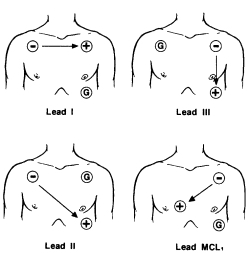
\includegraphics[width=0.4\textwidth]{ecg}
	\caption{Various positions for 3-lead EKG electrodes. Observe that the ground is not along the path of the electrical signal between the two charged electrodes. \cite{ecgpos} Image copied from RTBoard, \textit{Electrocardiography Devices}.}
\end{SCfigure}

\par Our design uses three electrodes to measure the electrical activity produced by the heart. By positioning two of the electrodes across the heart and the remaining one elsewhere on the body (not in between the two measuring electrodes) as a reference ground, we can generate a voltage across the skin over the heart. The resulting difference will be small, however, so we need an instrumentation amplifier to provide gain to render the signal interpretable. This amplified signal will be sent to an Arduino (Sparkfun Redboard). When connected to a computer, the Arduino's serial input can be recorded and graphed.

\section{PQRST}

\begin{SCfigure}[][htb!]
	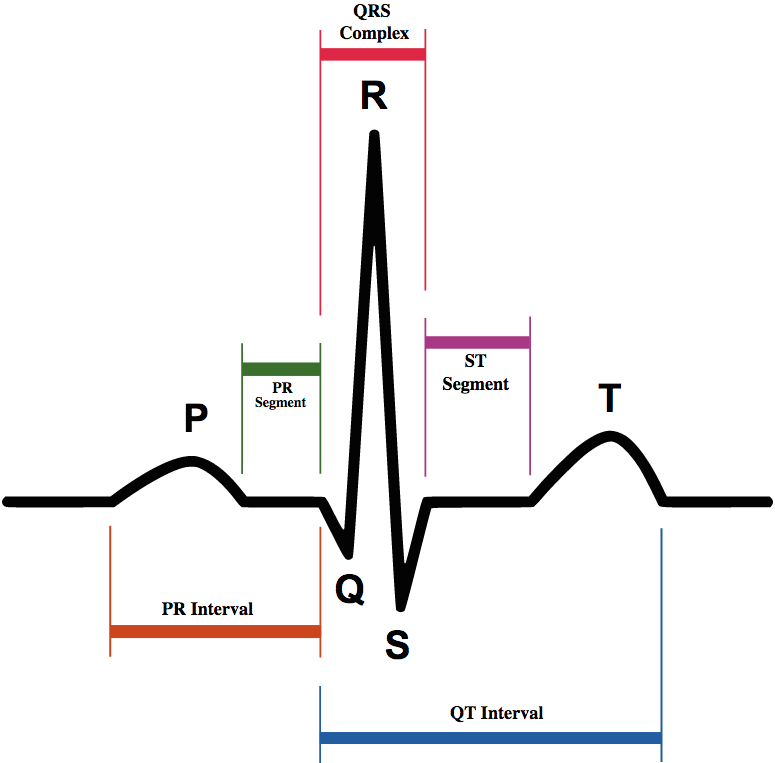
\includegraphics[width=0.4\textwidth]{PQRST}
	\caption{Schematic representation of an EKG reading.  The QRS complex represents the ventricular depolarization and contraction of the heart chambers. \cite{wikiimage} Image copied from Wikipedia article on Electrocardiography.}
\end{SCfigure}
	\onehalfspace

\par For this design we are looking to record the electrical signal of the heartbeat's QRS complex. The QRS complex is the combination of the three main graphical deflections observed on the electrocardiogram produced after the P and T wave. The P wave is the first short upward spike recorded in an ECG, and indicates the contraction of atria that pump blood into the ventricles. The QRS represents the ventricular depolarization and contraction, and it is graphed as a downward deflection, Q; a high upward deflection, spike R, and another downward S wave. Physiologically normal interval durations within the PQRST process happen quickly, in the order of tens of milliseconds. We expect a normal QRS interval to last around 60ms. Overall, we are looking for various contractions that occur in the heart and produce an electrical signal around 0.5mV. \cite{karptalk}

\par 
The baseline of the electrocardiogram is measured by the $\text{V}_{\text{ref}}$ terminal of the instrumentation amplifier. Due to variability in the baseline as a direct result of autonomous muscle contractions, however, we must process the baseline with a bandpass filter. Doing this in software will require post-processing (filtering the data after it has been collected), which we are currently achieving using the scipython bandpass filter module and the scipython notch filter. A bandpass filter is designed to remove any frequencies above frequency B $(f_B)$ and below frequency A $(f_A)$ where $f_A < f_B$. For the EKG, a bandwidth of $\sim$2.2 Hz from 0.8 to 3.0 Hz is optimal, as those parameters represent the normal range of the human heartbeat frequency (48 bpm to 180 bpm respectively), though we expect the signal to mostly consist of the 0.85 to 1.15 Hz bandwidth. The notch filter is an inversion of the bandpass filter in that it will filter out any frequencies between $f_A$ and $f_B$. In the EKG this filter will be used to remove the 60Hz noise produced by inductive capacitance of the surrounding (mains-level) electronics. Both filters will be imported from the SciPython module \cite{SciPython}    

The final data set will be fed into a graphing program, which will then output data to two modules, the Graphic User Interface (GUI) Module and the Diagnostic Reader Module (DRM). The DRM will also then output to the GUI. The GUI will be a highly simplified interface that will allow the user to change some of the parameters of the program to improve usability, possibly including bandpass filter parameter alterations and changing the DRM to better serve the needs of the user. 

\section{Design Problems}
Anything we may have encountered...
	\begin{itemize}[leftmargin=*]
		\item[] \textbf{Parts:}
			\begin{itemize} 
				\item Universal ECG EKG Electrodes Electrodes
				\item Sparkfun Redboard Arduino
				\item INA122 Instrumentation Amplifier
				\item LT1354 Operational Amplifier
				\item DC Filter
					\item C330C124KCR5TA Capacitor
					\item MRS25000C8253FRP00 Resistor
					\item HVR2500001004FR500 Resistor
				\item Wires
				\item Software Modules
					\item Registration Module
						\item Serial system in Arduino
					\item Pairing Module
					\item Noise Filter
						\item Bandpass Filter
						\item Notch Filter
					\item Grapher Module
						\item export to GNUplot
					\item Diagnostic Readout Module
						\item Heart Rate
						\item Peak Intervals
					\item GUI Module
					
			\end{itemize}
		\item[] \textbf{Education:}
			\begin{itemize}
				\item Complex Impedance basics 
				\item DC Filtering (High pass filtering?)
			\end{itemize}
	\end{itemize}
\pagebreak
\section{Circuit Design}
\begin{figure}[htb!]
\centering
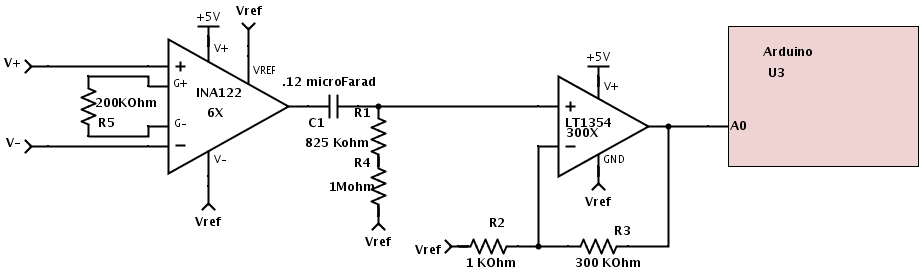
\includegraphics[width=\textwidth]{blockdiagnew}
\end{figure}
\begin{itemize}[leftmargin=*]

\item[] \textbf{Hardware Modules:}\\
	Human: Only prerequisite is a beating heart (and consent).\\
	Instrumentation Amplifier: Voltage fluctuations may be lower than the Arduino's resolution ($\geq$5mV), so we must use the amplifier to boost the signal to a level we can monitor. Since the signal will be approximately 0.5 mV, however, even small fluctuations at required gain ($\sim$5000x) could produced DC noise as high as 300 mV. \cite{karptalk} Therefore, any significant gain on the voltage in the instrumentation amplifier runs the risk of saturating (and thus overloading) it. As such, the primary purpose of the instrumentation amplifier will be to generate a differential signal, rather than to boost the voltage.\\
	Arduino: Converts analog input to digital output for Laptop using a serial output.\\
	Computer: Runs software/code and displays data. 
	
\item[] \textbf{Software Modules:}\\
	Register: Generates a list of differential values and time recorded, pairing the two values.\\
	Noise Filters:\\
		Bandpass Filter: Removes noisy frequencies higher and lower than the target bandwidth, imported from SciPython. \cite{SciPython}\\
		Notch Filter: Removes ~60 Hz noise generated by surrounding electronics.  
	Grapher: Plots all data points and connects to generate EKG waveform, imported from matplotlib\\
	GUI: Basic interface with ability to change graphing options and potentially activate/disable diagnostic screening or change diagnostic parameters manually.\\
	
\item[] \textbf{Hypothetical Software Module:}\\
	Diagnostic: Determines average distance between waveform peaks, possibly other diagnostically relevant information as well.
\end{itemize}

\section{Current Design Plans}
We plan on using a Texas Instruments INA122PA-ND instrumentation amplifier to boost the voltage differential from our electrodes. \cite{INA122PA-ND} Because the signal will be inverted, we will need to manipulate the signal further in software. The calculations are as follows\\
\noindent - Gain from INA122PA-ND is adjusted by changing shunt from gain resistor terminal to ground.\\
We will also include an analog bandpass filter composed of low- and high-pass filters. Because this filter's performance will depend on the data we gather, the circuit's specific components will be determined after sufficient signal information is gathered.

\section{Cost}
We are not considering manufacturing costs for now (e.g. solder, access to testing equipment) as these should be available to anyone with the skill necessary to assemble this device.

\noindent \textbf{Sparkfun Redboard:} \hfill \$20\\
\textbf{Breadboard TW-E40-1020:} \hfill \$8.98\\
\textbf{Wires:} \hfill \$4.95\\
\textbf{Texas Instruments INA122PA-ND:}  \hfill \$6.35\\
\rule{\textwidth}{1pt}
\textbf{Total Cost:} \hfill Including Shipping/Markup: \$46.50\\
\pagebreak

\begin{thebibliography}{11}

\bibitem{ecgpos}
"Electrocardiography Devices." Electrocardiography Devices. N.p., n.d. Web. 24 Feb. 2015. \\ \url{http://rtboardreview.com/public/equipment_room/ats_ecg.htm}

\bibitem{wikiimage}
Cardiac Waveform. Digital image. Electrocardiogram. \textit{Wikipedia}, n.d. Web. 24 Feb. 2015. \\ \url{http://en.wikipedia.org/wiki/Electrocardiography#mediaviewer/File:QRS_complex.png}.

\bibitem{howtoread}
"How to Read an Electrocardiogram (ECG). Part One: Basic Principles of the ECG. The Normal ECG." N.p., n.d. Web. 24 Feb. 2015. \\ \url{http://www.southsudanmedicaljournal.com/archive/may-2010/how-to-read-an-electrocardiogram-ecg.-part-one-basic-principles-of-the-ecg.-the-normal-ecg.html}.

\bibitem{karplus}
Karplus, Kevin. "Two-Stage EKG." Web log post. Gasstationwithoutpumps. Wordpress, 14 July 2012. Web. 17 Feb. 2015. \\ \url{https://gasstationwithoutpumps.wordpress.com/2012/07/14/two-stage-ekg/}.

\bibitem{karptalk}
Personal communication with Dr. Karplus regarding typical EKG sensor output.

\bibitem{INA122PA-ND}
Data sheet for Texas Instruments INA122PA-ND instrumentation amplifier. Web. March 1, 2015.\\ \url{http://www.ti.com/lit/ds/symlink/ina122.pdf}

\bibitem{SciPython}
Eric Jones and Travis Oliphant and Pearu Peterson and others. SciPy: Open source scientific tools for Python, 2001-present.March 1, 2015
\url{http://www.scipy.org/"}

\bibitem{matplotlib}
Hunter, J. D. Matplotlib: A 2D graphics enviroment.
Computing in Science \& Engineering vol.9 \#3 pg. 90-95
publisher: IEEE Computer Society, 2007. \url{http://matplotlib.org/index.html}



\end{thebibliography}

\end{document}  